%%%%%%%%%%%%%%%%%%%%% author.tex %%%%%%%%%%%%%%%%%%%%%%%%%%%%%%%%%%%
%%
%% sample root file for your "contribution" to a contributed volume
%%
%% Use this file as a template for your own input.
%%
%%%%%%%%%%%%%%%%% Springer %%%%%%%%%%%%%%%%%%%%%%%%%%%%%%%%%%
%
%
%% RECOMMENDED %%%%%%%%%%%%%%%%%%%%%%%%%%%%%%%%%%%%%%%%%%%%%%%%%%%
%\documentclass[graybox]{svmult}
%
%% choose options for [] as required from the list
%% in the Reference Guide
%
%\usepackage{mathptmx}       % selects Times Roman as basic font
%\usepackage{helvet}         % selects Helvetica as sans-serif font
%\usepackage{courier}        % selects Courier as typewriter font
%\usepackage{type1cm}        % activate if the above 3 fonts are
                            %% not available on your system
%%
%\usepackage{makeidx}         % allows index generation
%\usepackage{graphicx}        % standard LaTeX graphics tool
                             %% when including figure files
%\usepackage{multicol}        % used for the two-column index
%\usepackage[bottom]{footmisc}
%\usepackage{amsmath}
%
%% places footnotes at page bottom
%
%% see the list of further useful packages
%% in the Reference Guide
%
%\makeindex             % used for the subject index
                       %% please use the style svind.ist with
                       %% your makeindex program
%
%%%%%%%%%%%%%%%%%%%%%%%%%%%%%%%%%%%%%%%%%%%%%%%%%%%%%%%%%%%%%%%%%%%%%%%%%%%%%%%%%%%%%%%%%%
%
%\begin{document}

\title{Global optimization: from one-dimensional to multidimensional problems via the dimensionality reduction}
\titlerunning{Global optimization via dimensionality reduction}
% Use \titlerunning{Short Title} for an abbreviated version of
% your contribution title if the original one is too long
\author{Vladimir A.Grishagin and Yaroslav D.Sergeyev}
% Use \authorrunning{Short Title} for an abbreviated version of
% your contribution title if the original one is too long
\institute{Vladimir A.Grishagin \at N.I.Lobachevsky State University, Gagarin Avenue 23, 603950 Nizhni Novgorod, Russia   \email{vagris@unn.ru}
\and Yaroslav D.Sergeyev \at N.I.Lobachevsky State University, Gagarin Avenue 23, 603950 Nizhni Novgorod, Russia 
\at DIMES, University of Calabria, Via P. Bucci, Cubo 42-C, 87036 Rende (CS), Italy \email{yaro@si.deis.unical.it}}
%
\maketitle


\abstract{This paper is devoted to the basic statements and general definitions concerning the global optimization problems and algorithms. At the beginning, relevant notions are introduced and different statements of global optimization problems are described. As a main optimization statement, a non-linear programming problem is considered.  The concepts of numerical methods for solving the optimization problems are discussed and a general abstract model for successive methods is introduced. On the base of abstract description its algorithmic implementation (general computational scheme) is given. The model of sequential optimization expands for the case of parallel computations and general computational procedures for synchronous and asynchronous parallel methods are presented. Convergence of optimization methods and possibility of obtaining estimations of the problem solution after a finite number of objective function evaluations are discussed. Significant complexity of multidimensional multiextremal optimization problems is considered and approaches of overcoming this complexity via reduction schemes are briefly described. }

\section{The global optimization problem}
\label{sec:1_1}
The aim of this section is to introduce the necessary terms and to formulate the general problem of the global optimization, the investigation of which the present monograph is dedicated to. 
Let $\varphi(y)$ be a real-valued function, defined over a domain $D$ of the $N$-dimensional Euclidean space $R^N$ with a finite value at every point of $Q$.

Let us designate 
\begin{equation}
\label{eq:1_1_1}
\inf_{y\in Q}\varphi(y) \equiv\inf\{\varphi(y):y \in Q\}
\end{equation}
as the infimum of $\varphi(y)$ in the domain $Q$.
\begin{definition}
If there exists a point  $y^*\in Q$  such that 
\begin{equation}
\label{eq:1_1_2}
\varphi(y^*)=\inf\{\varphi(y):y \in Q\}
\end{equation}
then $\varphi(y)$ reaches its infimum in the domain $Q$, and $y^*$ is \textit {the global (absolute) minimum point} or \textit {the global minimizer}. The value $\varphi^* = \varphi(y^*)$ is the lowest or global optimum (minimum) value of $\varphi$ in $Q$ and is denoted as 
\begin{equation}
\label{eq:1_1_3}
\min_{y\in Q}\varphi(y) \equiv\min\{\varphi(y):y \in Q\}.
\end{equation}
\end{definition}
Let us denote the set of all points $y\in Q$  satisfying (\ref{eq:1_1_2}) as
\begin{equation}
\label{eq:1_1_4}
Q^*=Arg\min_{y\in Q}\varphi(y) \equiv Arg\min\{\varphi(y):y \in Q\}.
\end{equation}

Let us give one more important definition featuring the extremal properties of the functions.
\begin{definition} 
A point $y'$  is called a \textit {local minimum point} in the domain $Q$ if there exists such number $\epsilon>0$ that for all $y \in Q$ satisfying the inequality $\left\|y-y'\right\|$ the condition $\varphi(y')<\varphi(y)$ is true.
\end{definition}
The functions with several local minima in the domain $Q$ are called the \textit {multiextremal} ones in this domain, and those with a single local minimum are called the \textit {unimodal (uniextremal)} functions. Obviously, any global minimum is a local one, and for a unimodal function its unique local minimum is the global one.
In the optimization models related to the analysis of the function $\varphi(y)$, different formalizations of the desired solution are possible and, as a result, different optimization problem statements arise. In this connection, let us give a classification of such problem statements in the following formulations.
\begin{definition} 
Let us treat the optimization problem as a problem of the following kind: to find the predefined extremal characteristics of the function $\varphi(y)$ over the domain $Q$.
\end{definition}
Various optimization problem statements are possible subject to the desired extremal characteristics.

\textbf{Problem Statement A.} Find the infimum of the function $\varphi(y)$
\begin{equation}
\label{eq:1_1_5}
\varphi^*=\inf\{\varphi(y):y \in Q\}.
\end{equation}

\textbf{Problem Statement B.} Find the infimum from (\ref{eq:1_1_5}) and if the set of the global minimum points from (\ref{eq:1_1_2}) is not empty, find at least one point $y^*=Q^*$.

\textbf{Problem Statement C.} Find the infimum from (\ref{eq:1_1_5})  and all global minimum points (or make sure that the set $Q^*$ is empty).

\textbf{Problem Statement D.} Find all coordinates and values of all local minima of the function $\varphi(y)$ in the domain $Q$.

The problem statements A--D are related to the finding of the global minimum, but sometimes the following problem statement is used even for the multiextremal functions:

\textbf{Problem Statement E.} Find a local minimum of the function $\varphi(y)$ in the domain $Q$.

The optimization problem statements A--E are the most commonly used (see, for example, classical monographs \cite{1_FloudasPardalos, 1_Himmelblau, 1_HorstPardalos, 1_HorstTuy, 1_McCormick, 1_Mockus, 1_Pinter,  1_SergKvasMonogr, 1_StrSergMon2000, 1_ZhigZhil}), although other variants are possible as well, for example, those given in \cite{1_Himmelblau}. The desired extremal characteristics defined by the problem statement $Z\in\{A, B, C, D, E\}$ are referred to as $Z$-solution of the optimization problem.

Let us denote the general optimization problem symbolically in the following form:
\begin{equation}
\label{eq:1_6}
\varphi(y)\rightarrow\inf, y \in Q.
\end{equation}

This problem is rather often referred to as the problem of the \textit{mathematical programming}.

If it is necessary to concretize the problem statement to be considered, we will specify the relevant desired $Z$-solution of the problem.

As  the supremum of a function $\varphi(y)$ in a domain $Q$ is connected with the infimum of the function $-\varphi(y)$ according to  the expression
\begin{displaymath}
\sup\{\varphi(y):y \in Q\} = -\inf\{-\varphi(y):y \in Q\}
\end{displaymath}
the problem of finding the extremal characteristics related to the maximum of the function $\varphi(y)$ (the maximization problem), can be reduced to the problem of the minimization of the function $-\varphi(y)$. Therefore, hereinafter the optimization problem will be considered in the form (\ref{eq:1_6}). The function $\varphi(y)$ in (\ref{eq:1_6}) will be called \textit{the objective function, the minimized function, or the optimized function},  the domain $Q$ will be called \textit{the feasible (admissible) domain}, and the elements of the set $Q$ will be called \textit{the feasible points}.

Let us denote the problem (\ref{eq:1_6}), for which the set of the global minimum points $Q^*$ is known to be nonempty a priori (the sufficient conditions for the non-emptiness of $Q^*$ are given, for example, by Weierstrass theorem), as
\begin{equation}
\label{eq:1_7}
\varphi(y)\rightarrow\min, y \in Q.
\end{equation}

Note that the mathematical programming problem is often formulated just in this form, although, of course, the problem (\ref{eq:1_6}) is the more general one. Let us reformulate the problem (\ref{eq:1_7}) in the form of a non-linear programming problem
\begin{equation}
\label{eq:1_8}
\varphi(y)\rightarrow\min, y \in Q\subseteq R^N,
\end{equation}
\begin{equation}
\label{eq:1_9}
Q=\{y \in D:g_j(y)\leq 0,1\leq j\leq m \},
\end{equation}
\begin{equation}
\label{eq:1_10}
D=\{y \in R^N:y_i\in [a_i,b_i],1\leq i\leq N \},
\end{equation}
i.e., the problem of finding the extremal values (in terms of the Problem statements A-D) of the objective (minimized) function $\varphi(y)$  over the domain $Q$ is defined by the \textit{coordinate} (\ref{eq:1_10}) and \textit{functional} (\ref{eq:1_9}) \textit{constraints} on the selection of feasible points (or vectors) $y=(y_1,\ldots ,y_N)$ . In this model, the constants $a_i,b_i, 1\leq i\leq N$,  determine the limits for the variation of the problem parameters (the components of the vector $y$), and are finite or (when the corresponding upper or/and lower limits are absent for some of them) they are assumed to be equal to $a_i=-\infty $  and/or $b_i=+\infty $.

Often, the constraints in the form of equations are also included in the non-linear programming problem statement. However, any equation $h(y)=0$ , first, could be represented formally as the system of two inequalities $h(y)\leq 0$  and $h(y)\geq 0$ . Second, in numerical solving an optimization problem on a computer the exact calculation of the equality $h(y)=0$ is often impossible, therefore, this equality is assumed to be computed  with some error $\delta>0$ , i.e., the inequality $\left|h(y)\right|\leq \delta$ is considered instead of the equation $h(y)=0$. Thus, taking into account the above reasons, one can claim that (\ref{eq:1_8})--(\ref{eq:1_10}) is the statement of  \textit {the general  problem of the nonlinear programming}.

If $m=0$ , i.e., there are no functional constraints, it is considered that $Q=D$. The problem (\ref{eq:1_8})--(\ref{eq:1_10}) in this case will be called \textit {the unconstrained optimization problem}.

Let us consider an optimization problem  for the function
\begin{displaymath}
%\label{eq:1_12}
\varphi(y_1,y_2)=-1.5y_1^2\exp(1-y_1^2-20.25(y_1-y_2)^2)-
\end{displaymath}
\begin{displaymath}
%\label{eq:1_12}
-(0.5(y_1-1)(y_2-1))^4\exp(2-(0.5(y_1-1))^4-(y_2-1)^4)
\end{displaymath}
within the domain $0 \leq y_1\leq 4,\ \  -1\leq y_2\leq 3$, with the following constraints 
\begin{displaymath}
g_1(y_1,y_2)=0.01((y_1-2.2)^2+(y_2-1.2)^2-2.25)\leq 0,
\end{displaymath}
\begin{displaymath}
g_2(y_1,y_2)=100(1-(y_1-2)^2/1.44-(0.5y_2)^2)\leq 0,
\end{displaymath}
\begin{displaymath}
g_3(y_1,y_2)=10(y_2-1.5-1.5\sin(6.283(y_1-1.75)))\leq 0,
\end{displaymath}
as a particular example.

\begin{figure}[t]
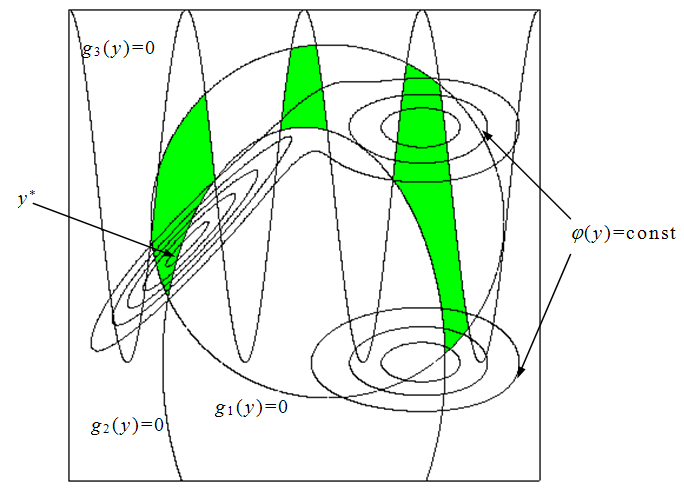
\includegraphics[width=0.7\linewidth]{figures/figure1_1.png}
\caption{Example of a global optimization problem with disconnected admissible domain}
\label{1_fig_1}    
\end{figure}

The set of the points satisfying the first constraint represents the circle with the boundary defined by the equation $g_1(y_1,y_2)=0$. The points satisfying the second constraint are located outside the ellipse defined by the equation $g_2(y_1,y_2)=0$. The points satisfying the third constraint are below the sinusoid $g_3(y_1,y_2)=0$. Thus, the feasible domain is disconnect and consists of three non-convex subdomains (the feasible domain is dark in Fig.~\ref{1_fig_1}). The global minimum $\varphi(y_1^*,y_2^*)=-1.489$  is achieved at the point $(y_1^*,y_2^*)$  = (0.942, 0.944).

\section{Numerical optimization methods}
\label{sec:1_2}

\subsection {Concept of algorithm. Sequential scheme}
\label {subsec:1.2.1}

Having stated the minimization problem, we now must answer the principal question: how to solve it?

The classical approach of the mathematical analysis suggests the following procedure for the analytical solution of the problem. Let us consider the one-dimensional case and assume that $\varphi(y)$ is a single argument function, which is piecewise smooth over the interval $[a,b]$. Then, the minimum of $\varphi(y)$ in $[a,b]$ can be achieved only at the points, where the derivative $\varphi'(y)=0$ , or where the derivative is discontinuous, or at the boundary points. Therefore, it is necessary to find all these points and to select from them the point with the lowest value. In other words, in order to solve the problem by this method, the following requirements should be satisfied:
\begin{enumerate}
\item{it is necessary to know the analytical formula for the function;}
\item{the function should be piecewise smooth;}
\item{the calculation of the derivative should be possible;}
\item{it is necessary to solve the equation $\varphi'(y)=0$;}
\item{the information on the derivative discontinuity points or a method for finding these ones are required.}
\end{enumerate}

Unfortunately, these requirements are fulfilled rarely. In the typical cases, the function $\varphi(y)$ is defined algorithmically, i.e., in the form of some calculation scheme, when one can calculate the value of $\varphi(y)$ at a given point y only (black-box function). In this case, the analytical investigation methods are unsuitable. Note that even if the function is defined analytically and if the derivative calculation is possible the initial problem (\ref{eq:1_6}) is reduced to the problem of finding all the derivative roots, the difficulty of which is comparable with the minimization problem.

The limited applicability of the analytical methods has caused the development and wide application of \textit {the numerical methods (algorithms)} for solving the optimization problems. Various definitions of the numerical optimization method have been given by many authors. The consideration of the method as an iteration procedure, which calculates certain characteristics of the minimized function at some points of the search domain is a common feature of all formulations. The calculated characteristics can include the value of the objective function, its gradient, the second derivatives matrix, etc. Let us denote the calculation of the function characteristics at a point as \textit {a search trial} and the set of the values of the function characteristics as \textit {a trial result}.

Hereinafter we will consider the function value at the trial point as the trial result. If an algorithm is executed on a single processor computer, the computing scheme of the algorithm consists of a series of operations executed sequentially, and all the trials are performed sequentially, i.e., we deal with a pure sequential numerical method. 

Let us give a formal definition of sequential optimization algorithm based on the methodology of the theory of operations research, or, more general, on the computational model for solving the problem (\ref{eq:1_6}). The generalization of this model onto the parallel computing case will be given in Subsect. \ref{subsec:1.2.2}

The development of a computational model presupposes an availability of some a priori information on the problem to be solved (before the beginning of the computations). This information could be obtained from the physical meaning of the problem or description of the properties of the model-based object. This information can include such properties of $\varphi(y)$ as continuity, smoothness, monotonicity, convexity, etc. The available information provides the researcher with the basis to attribute the problem (in our case, the function $\varphi(y)$ to a specific set (or class) $\Phi$. After the class $\Phi$ has been identified, the information known to the researcher a priori consists in the knowledge that the problem belongs to the class $\Phi$.

The selection of an \textit {optimization algorithm} (method for solving  the optimization problem) is the next important step in the computational model development. In the most general form, a numerical method $s$ for solving the problem from the class $\Phi$ is a set  (tuple) (\cite{1_StrMonRus})
\begin{equation}
\label{eq:1_11}
s=\left\langle \{G_k\},\{E_k\},\{H_k\}\right\rangle
\end{equation}
where 

-  $\{G_k\}$	  is a set of functionals defining the rules for the trial points selection \textit {(algorithm's decision rules)}, $k=1,2,\ldots$ ;

-  $\{E_k\}$	  is a set of functionals defining the rules of constructing the approximate solution (the estimates of extremum), $k=1,2,\ldots$ ;

-  $\{H_k\}$	  is a set of functionals defining the rules of stopping the computational process,  $k=1,2,\ldots$.

The order of the trial execution or the computational scheme of the algorithm   can be realized in accordance with the following steps.

\begin{description}[\textbf{Step 1}]
\item[\textbf{Step 1}]{The point 
\begin{equation}
\label{eq:1_12}
y^1=G_1(\Phi) \in Q
\end{equation}
is selected as the first trial coordinate and the trial counter $k=1$ .}
\item[\textbf{Step 2}]{Assume that the point of the $k$-th trial $y^k\in Q$  $(k\geq 1)$ has been selected. The value of the function $z^k=\varphi(y^k)$  is computed. Afterwards there is the following \textit {search (a posteriori) information} about the function $\varphi(y)$:
\begin{equation}
\label{eq:1_13}
\omega_k=\{(y^1,z^1),(y^2,z^2),\ldots ,(y^k,z^k)\}.
\end{equation}
This information allows reducing the class, which the function  $\varphi(y)$ belongs to, up to the set
\begin{equation}
\label{eq:1_14}
\Phi(\omega_k)=\{\psi\in\Phi:\psi(y^i)=z^i,1\leq i \leq k\}.
\end{equation}
}
\item[\textbf{Step 3}]{The current estimate 
\begin{equation}
\label{eq:1_15}
e^k=E_k(\Phi,\omega_k)
\end{equation}
of the extremum sought (approximate solution) is determined.}
\item[\textbf{Step 4}]{The next trial point 
\begin{equation}
\label{eq:1_16}
y^{k+1}=G_{k+1}(\Phi,\omega_k)
\end{equation}
is computed.}
\item[\textbf{Step 5}]{The number 
\begin{equation}
\label{eq:1_17}
h^k=H_k(\Phi,\omega_k,y^{k+1})\in \{0,1\}
\end{equation}
taking one of two possible values: 0 or 1 is determined. If $h^k=1$ the trial counter $k$ is increased by 1, and the return to the Step 2 of the scheme is carried out. If $h^k=0$ the computations are terminated, and the estimate $e^k$  is taken as the problem solution.}
\end{description}

The general computation model has been described. 

\example {Let us consider the simplest method of solving a one-dimensional problem (\ref{eq:1_6}) within an interval $[a,b]$, namely, the method of scanning  the function values in the nodes of a regular grid. The method consists in the partitioning of the search interval $[a,b]$ into $q$ equal parts. The function values are calculated at the points (nodes) of the partitioning, including the ends of the search interval. The lowest calculated value (and its coordinate, if it is required by the problem statement) is considered to be the solution of the problem. }

The computability of the function at any point of the search domain is sufficient for the applicability of the method. So, the class of the functions defined over the interval $[a,b]$ and being computable at every point of the interval can be considered as the a priori known class $\Phi$. 

For this method
\begin{displaymath}
G_1(\Phi)=a, G_{k+1}(\Phi,\omega_k)=a+k\frac{b-a}{q}, k\geq 1,
\end{displaymath}
\begin{displaymath}
  H_k(\Phi,\omega_k) =
  \begin{cases}
    0, & k > q, \\
    1, & k \leq q,
  \end{cases}
\end{displaymath}
\begin{equation}
\label{eq:1_18}
e^k=\varphi_k^*,
\end{equation}
where
\begin{equation}
\label{eq:1_19}
\varphi_k^*=\min_{1\leq i\leq k} \varphi(y^i),
\end{equation}
or
\begin{displaymath}
e^k=(\varphi_k^*,y_k^*),
\end{displaymath}
where 
\begin{displaymath}
%\label{eq:1_19}
y_k^*=\arg \min_{1\leq i\leq k} \varphi(y^i).
\end{displaymath}


\subsection {Parallel optimization algorithms}
\label {subsec:1.2.2}
The computational scheme (\ref{eq:1_12})--(\ref{eq:1_17}) implies  the sequential execution of all the algorithm steps, that can be provided by the single processor computers. But if a multiprocessor computer is available, a parallelization of the computational scheme and, therefore, an acceleration of the optimization process can be realized. The parallelization of optimization methods could be done in several ways. It is possible to parallelize, in the first place, the calculation of the objective function, secondly, the implementation of the rules $G_k,E_k,H_k$ , and, finally, the scheme (\ref{eq:1_12})--(\ref{eq:1_17}) providing simultaneous execution of several trials. However, the parallelization of the objective function describing the optimized object is specific for different objective function models, and as a matter of fact, cannot be related to the general optimization scheme. The parallelization of the functionals  $G_k,E_k,H_k$ depends essentially on the class of algorithms. Besides, often these functionals are rather simple, and their parallelization is just of no use. Therefore, the subject of the consideration in the present subsection  is the consideration of some \textit {fundamental principles} for a parallel execution of trials.  Let us use the term \textit {iteration} for the simultaneous (parallel) execution of several trials (each trial is executed by a separate processor). Let us denote the number of trials during the $n$-th iteration as $p(n)$ , and the total number of trials executed during all $n$ iterations as $k(n)$ . In other words, we assume that we have  $p$  processors at our disposal while executing the $n$-th iteration. Actually, the number of processors employed can be different for different iterations. 

Let us consider the synchronous variant of the parallelization, where the transition to the next iteration is performed after full termination of the current one, i.e., after completing the last trial of the current iteration. In this case, it is obvious that $k(n)=p(1)+\ldots + p(n), \; n\geq 1$.  Let us denote the vector of the trial coordinates at the $n$-th iteration as $u(n)$ , i.e.,
\begin{displaymath}
u(n)=(y^{k(n-1)+1},\ldots ,y^{k(n)}) .
\end{displaymath}
and the first $j$ coordinates of the vector $u(n)$  as $u_j(n)$ , i.e., 
\begin{displaymath}
u(n)=(y^{k(n-1)+1},\ldots ,y^{k(n-1)+j}),\ 1\leq j\leq p(n) .
\end{displaymath}

Then, the general computational scheme of a synchronous parallel optimization algorithm can be written as follows.

\paragraph{\textbf{Synchronous parallel algorithm scheme}}
\begin{description}[\textbf{Step 1}]
\item[\textbf{Step 1}]{Set the iteration number $n=1$  and the initial number of trials $k(0)=0$ . Select $p(1)$ points of the first iteration  
\begin{equation}
\label{eq:1_20}
y^1=G_1(\Phi)\in Q,y^i=G_i(\Phi,u_{i-1}(1))\in Q,\ 2\leq i\leq p(1)
\end{equation}
and assign the number of trials $k(1)=p(1)$.}
\item[\textbf{Step 2}]{Assume that the points of the $n$-th iteration $u(n),\ n\geq 1,$ , have been obtained. The computations of the objective function values $z^j=\varphi(y^j)$,   $\ k(n-1)+1\leq j\leq k(n)$, are executed (each value is computed by a separate processor). After computing all the values there is the following search information on the function $\varphi(y)$ (\textit{a posteriori information}):
\begin{equation}
\label{eq:1_21}
\omega_k=\omega_{k(n)}=\{(y^1,z^1),(y^2,z^2),\ldots ,(y^{k(n)},z^{k(n)})\}.
\end{equation}
As before, the new information (\ref{eq:1_21}) allows one to reduce the class, which the function $\varphi(y)$ belongs to, up to the set   
\begin{equation}
\label{eq:1_22}
\Phi(\omega_{k(n)})=\{\psi\in\Phi:\psi(y^i)=z^i,1\leq i \leq k(n)\}.
\end{equation}
}
\item[\textbf{Step 3}]{After completing all the trials within the current iteration, the estimate of the extremum (an approximate solution) is formed:  
\begin{equation}
\label{eq:1_23}
e^{k(n)}=E_{k(n)}(\Phi,\omega_{k(n)}).
\end{equation}
}
\item[\textbf{Step 4}]{Coordinates of the trials at the ($n+1$)-th iteration are computed:
\begin{equation}
\label{eq:1_24}
\begin{gathered}
y^{k(n)+1}=G_{k(n)+1}(\Phi,\omega_{k(n)}) \\
y^{k(n)+i}=G_{k(n)+i}(\Phi,\omega_{k(n)},u_{i-1}),\  2\leq i\leq p(n+1),
\end{gathered}
\end{equation}
and the number of the search trials $k(n+1)=k(n)+p(n+1)$  is set.}
\item[\textbf{Step 5}]{The number 
\begin{equation}
\label{eq:1_25}
h^{k(n)}=H_{k(n)}(\Phi,\omega_{k(n)},u(n+1))\in \{0,1\}
\end{equation}
taking one of two possible values: 0 or 1 is determined. If $h^{k(n)}=1$ the iteration counter $n$ is incremented ($n=n+1$), and the return to the Step 2 of the scheme is carried out. If $h^{k(n)}=0$ the  iterations are completed, and the estimate $e^{k(n)}$  is taken as the (approximate) problem solution.}
\end{description}
\note {In the proposed scheme it is assumed implicitly, that the numbers   of the processors involved into the execution of a particular step of the algorithm  are known a priori for all iterations. At the same time, the scheme can be easily supplemented with a processor number selection rule in dependence on the current search state, if to introduce a functional $P_n(\Phi,\omega_{k(n-1)})$  such that}
\begin{displaymath}
p(n)= P_n(\Phi,\omega_{k(n-1)}).
\end{displaymath}

Then, Step 4 of the computational scheme can be written as follows. 
\begin{description}[\textbf{Step 4}]
\item[\textbf{Step 4}]{The number of processors required for the execution of the  $(n+1)$-th iteration 
\begin{displaymath}
p(n+1)= P_{n+1}(\Phi,\omega_{k(n)}).
\end{displaymath}
is determined and $p(n+1)$  trial coordinates of the current iteration are calculated according to (\ref{eq:1_24}).}
\end{description}

Let us consider again the method of scanning  a function $\varphi(y)$ in the nodes of a regular grid to illustrate a parallel algorithm. Let us assume for simplicity that the number of processors $p$ is the same for all iterations, that the number of nodes $q>p$  and is divisible by $p$. Then, the decision rules $G(\bullet )$  in the expressions (\ref{eq:1_20}) and (\ref{eq:1_24})  obviously take the form 
\begin{displaymath}
G(\bullet )=a+(j-1)\frac{b-a}{q},\ k(n)+1\leq j\leq k(n)+p(n+1),
\end{displaymath}
and the estimate of extremum and the condition of termination remain the same to those in the sequential prototype. 

The synchronous scheme considered here has a drawback that the processors completed their trails within current iteration earlier than other ones, stay idle waiting for the completion of the iteration. Let us consider the computational scheme of an \textit{asynchronous} parallel optimization algorithm, which is free from this disadvantage. In the asynchronous algorithm the iterations become distributed in time. Therefore, it is convenient to deal with the number of trials $k$. Thereby, let us introduce a set of completed trials  $w(k)=\{w_1,w_2,\ldots,w_k\}$  and a set  of coordinates $v(k)=\{v_1,v_2,\ldots,v_{p(k)}\}$ , at which new trials are executed after completing the preceding $k$ trials. Here $p(k)$ is the number of processors executing the current trials, and $w_j=y^{i_j},\ 1\leq j\leq k,\ v_s=y^{i_s},\ 1\leq s\leq p(k), 1\leq i_j,i_s \leq k+p(k)$ . It is obvious, that $w(k)\cup v(k)=\{y^1,\ldots,y^k,\ldots,y^{k+p(k)}\}$ .

Let us assume for simplicity, that we have  $p\geq 2$  processors at our disposal for execution of the algorithm, and this number remains constant in the course of optimization. A variant of the computational scheme with a different number of processors for different search steps can be obtained easily by generalization of the proposed asynchronous scheme consisting in the following.
\paragraph{Asynchronous parallel algorithm scheme}
\begin{description}[\textbf{Step 1}]
\item[\textbf{Step 1}]{First $p$ points of initial trials are selected according to the decision rules $G_i(\bullet ),\ 1\leq i\leq p$ :  
\begin{equation}
\label{eq:1_26}
\begin{gathered}
y^1=G_1(\Phi\in Q), \\
y^i=G_i(\Phi,y^1,\ldots,y^{i-1)}\in Q,\ 2\leq i\leq p,
\end{gathered}
\end{equation}
the vector $v(0)$  with the components $v_i=y^i,\;1\leq i\leq p$, is formed, and the number of trials $k=0$ is set.}
\item[\textbf{Step 2}]{Wait for the completion of trials by one or several processors. Assume that $1\leq \pi=\pi(k)\leq p$  processors have completed the computation of the function values $z^{i_j}=\varphi(y^{i_j})$  at the points $y^{i_1},\ldots,y^{i_\pi}, y^{i_j}\in v(k),\ 1\leq j\leq \pi$. Then, assign $k=k+\pi$, form the set $w(k)=w(k-\pi)\bigcup \{y^{i_1},\ldots,y^{i_\pi}\}$  and the set $v(k)$ removing from the set $v(k-\pi)$  points $y^{i_1},\ldots,y^{i_\pi}$ . Afterwards there is the following search information on the function $\varphi(y)$ \textit{a posteriori}:
\begin{equation}
\label{eq:1_27}
\omega_k=\{(y^{i_1},z^{i_1}),(y^{i_2},z^{i_2}),\ldots ,(y^{i_k},z^{i_k}\}.
\end{equation}
where  $y^{i_s}\in w(k),z^{i_s}=\varphi(y^{i_s}),\;1\leq s\leq k$.
}
\item[\textbf{Step 3}]{The current estimate (approximate solution) of the extremum is determined as  
\begin{equation}
\label{eq:1_28}
e^k=E_k(\Phi,\omega_k).
\end{equation}
}
\item[\textbf{Step 4}]{
\begin{equation}
\label{eq:1_29}
\begin{gathered}
y^{k+1}=G_{k+1}(\Phi,\omega_{k}) \\
y^{k+i}=G_i(\Phi,\omega_k,y^{k+1},\ldots,y^{k+i-1}),\;2\leq i\leq \pi,
\end{gathered}
\end{equation}
are computed and added to the set $v(k)$.} 
\item[\textbf{Step 5}]{The number 
\begin{equation}
\label{eq:1_30}
h^k=H_k(\Phi,\omega_k,y^{k+1},\ldots,y^{k+\pi})\in \{0,1\}
\end{equation}
taking one of two possible values: 0 or 1 is computed. If $h^k=1$, switching to Step 2 of the current scheme is carried out. If $h^k=0$, the computations should be completed and the current estimate $e^k$  is taken as the problem solution.}
\end{description}

Some examples of both the synchronous and asynchronous optimization algorithms are presented can be found in this monograph (see \cite{1_BarGerStrChap4, 1_BarGerStrChap6, 1_GriIsrChap5, 1_GriSergChap3}).
\subsection {Convergence and estimates of extremum}
\label {subsec:1.2.3}
Thus, when solving a minimization problem for a function  $\varphi(y)$ any search method generates a sequence of trial coordinates (or just the trial sequence) $\{y^k\}=y^1,y^2,\ldots,y^k,\ldots$  (where $y^k$   is the coordinate of the $k$-th trial) as well as a sequence of trial results $\{z^k\}=z^1,z^2,\ldots,z^k,\ldots$ . Remind, that as trial results we consider the objective function values, i.e., $z^i=\varphi(y^i),\;i=1,2,\ldots$ .    

The behavior of the method is determined via the properties of sequences  $\{y^k\}$ and  $\{z^k\}$. Therefore, the investigation of the search method could be carried out by means of a study of trial sequences which it generates. 

Thereby, let us ask the question: what requirements should be imposed to trial sequences of a numerical optimization method? Of course, the main requirement is that execution of the trials at the points $\{y^k\}$  with the trial results $\{z^k\}$  could provide a solution of the problem, i.e., finding the solution corresponding to the selected problem statement. At the same time, since a computer can execute a finite number of trials only, it is desirable to obtain the exact solution after constructing a finite sequence $\{y^k\}$. Unfortunately, such a favorable situation takes place in rare and simple cases only, for example, in the linear programming problems. Therefore,  an asymptotically exact assessment is interesting often, and an infinite trial sequence is considered (in this case for the introduced  optimization method models in (\ref{eq:1_17}) , (\ref{eq:1_25}), (\ref{eq:1_30}) $H_k=1$  for any $k\geq1$, i.e., in fact, the termination criterion is absent). In other words, this sequence is required to converge to the exact problem solution. Since in the problem statements $B-D$ the desired solution may include several minimum points, we will understand the convergence of a method in the sense of the following definition.
\begin{definition} 
\label{def:1_4}
The trial sequence $\{y^k\}$  converges to the solution of the problem (\ref{eq:1_6}) defined by the corresponding problem statement, if:
\begin{enumerate}
\item{it includes a subsequence  $\{\bar{y}^k\}$, for which $\lim_{k \to \infty}\bar{y}^k=\varphi^*$;}
\item{in the case when the solution includes one or several minimum points, for each such point there exists a subsequence of the sequence $\{y^k\}$  converging to it.}
\end{enumerate}
\end{definition}
Trial sequence converging to the exact solution of the problem statement $Z \in \{A,B,C,D,E\}$ is called the minimizing sequence for the problem statement $Z$ or $Z$-minimizing sequence. The term «minimizing sequence» was introduced in \cite{1_Vasiliev} and corresponds to the concept of $A$-minimizing sequence.

Now we would like to pay the reader’s attention to the following important aspect. The property of convergence in the theory of the extremum search methods attracts significant attention, since the asymptotics provides a potential possibility to obtain the exact solution with any predefined accuracy after a finite number of trials. However, this possibility itself is not sufficient for the practical implementation of the methods. In addition, it is necessary to know how to determine a proximity measure of the obtained approximate solution to the exact one, i.e., how to estimate the error of the problem solution using the finite number of trials.

Let us consider the following simple example. Let the class $\Phi$ consist of the continuous one-dimensional functions, defined over the interval $Q=[a,b]$, i.e., it is known a priori that the minimized function $\varphi(y)$ is continuous in the domain $Q$. Assume that the values of the function $\varphi(y)$ are calculated in a finite number of points   What is it possible to say about the coordinate of the global minimum after that? Whatever points $y^1,y^2,\ldots,y^k$  and values $z^1,z^2,\ldots,z^k$ were obtained after $k$  trials, for any point $y^*\in Q \ \ (y^*\notin \{y^1,y^2,\ldots,y^k\})$   a continuous function passing through the points $(y^i,z^i),1\leq i\leq k$,  i.e., belonging to the class $\Phi(\omega_k)$ from (\ref{eq:1_14}) and providing the global minimum at the point $y^*$  with any predefined value
\begin{displaymath}
\varphi^*<\min_{1\leq i\leq k} z^i 
\end{displaymath}
can be built always. For example, an interpolation polynomial of the $k$-th power, passing through the points  $(y^i,z^i),1\leq i\leq k,$ and the point $(y^*,\varphi^*)$, could be taken as such function.

All the above means that no conclusions on the position of the global minimum point can be drawn after any  finite number of trials. Similarly, the only conclusion on the value $\varphi^*$  of the global minimum can be as follows:
\begin{displaymath}
\varphi^*\leq \varphi_k^*, 
\end{displaymath}
where $\varphi_k^*$  is determined by (\ref{eq:1_19}). Therefore, it is impossible to estimate the value 
\begin{displaymath}
\epsilon_k=\left|\varphi^*-\varphi_k^*\right|, 
\end{displaymath}
i.e., the accuracy of the program solution.

The possibility to obtain the estimates of the extremum based on a finite number of trials depends on the properties of the function class, which the minimized function belongs to, or, in other words, on the information about the function $\varphi(y)$ known a priori. In fact, only two broad classed of the functions allow building such estimates: the class of one-dimensional unimodal functions and the class of the functions satisfying Lipschitz condition (in the general case of the multidimensional and multiextremal functions).

The availability of the extremum estimates built on the base of a finite (truncated) trial sequence allows (in some cases) formulating and solving the problem of theoretical design of the optimal (in different meanings) optimization methods (see, for example, \cite{1_Kushner, 1_Mockus, 1_StrSergMon2000, 1_Sukharev1971, 1_Sukharev1972, 1_Sukharev1989}) . This interesting problem falls out of the scope of the present paper. However, the availability of the extremum estimates is important for the investigation of the parallelization efficiency of the optimization methods.

\section{Multiextremal problems and reduction of complexity}
\label{sec:1_3}
In multiextremal problems the dimension affects the difficulty of solving such problems significantly. For example, for the class of the functions satisfying Lipschitz condition so called  \textit{curse of dimensionality} consisting in the exponential growth of the computational costs with increasing dimensionality takes place. Namely, if $p$ evaluations of the objective function are required to achieve the solution accuracy $\epsilon$ in the one-dimensional case, in the $N$-dimensional problem $\alpha p^N$  trials are required to achieve the same accuracy. Here the coefficient $\alpha$ depends on the objective function, on the feasible domain, and on the method used. 

For particular small classes of the multiextremal problems the computational cost growth rate can be slower than the exponential one. For example, for the separable functions minimized over a hyperinterval $D$ the computational costs grow linearly. This fact demonstrates that increase of the efficiency of optimization methods is possible by a thorough accounting for the a priori known information only. Designing the efficient optimization methods as optimal decision rules based on the minimax or Bayesian approach to the concept of optimal methods of the extremum search within the frameworks of the respective mathematical models can be a form of such accounting. Unfortunately, the problem of building the optimal algorithm for the multidimensional multiextremal functions is  very complicated and connected with solving the problems of the covering theory of the feasible domain (see, for example, \cite{1_Sukharev1971, 1_Sukharev1972, 1_Sukharev1989}).

Another approach to the design of the numerical methods for the analysis of the multidimensional multiextremal problems exploits the idea of \textit{the complexity reduction} where the solution of the initial problem is replaced with solving one or several simpler problems.

One of such reduction schemes is based on the elementary fact that the global extremum is a local one. Hence the clear conclusion follows that in order to find the global optimal solution it is sufficient to find all local minima and to select the lowest of them. In the context of the theoretical approach this construct seems to be a perfect one. However, in practice some difficulties arise. 
First of all, the following question arises: how to find all local minima? This problem can be solved, if for each local minimum its attraction zone, i.e., such neighborhood of the minimum point, in which the function is unimodal, is known. Then, having positioned the initial search point into this neighborhood, one can find the desired local minimum by some local method. In other words, this scheme implies a subdivision of the search domain into the local minimum attraction zones to be known. However, in practice such information is absent a priori as a rule (even the number of local extrema is unknown usually). Therefore, an additional problem of the starting point selection arises when applying this approach. 

The simplest method consists in the selection of the starting points using the Monte-Carlo method scheme (see, for example, the fundamental monograph \cite{1_ZhigZhil}), i.e., randomly according to some distribution in the search domain (usually, the uniform one) or in using the nodes of a regular grid as the starting points.

The convergence to the global extremum in this method is provided by the fact that if to increase the number of the starting points at least one of them will fall into the global extremum attraction zone since these grids (either regular or random) are built to provide a coverage of the whole search domain with increasing density. However, this scheme has an essential drawback. As a matter of fact, several starting points can fall into the attraction zone of a local minimum, i.e., this particular local minimum will be found several times. Different schemes have been proposed to overcome this disadvantage ( see \cite{1_BetroSchoen, 1_BoendeRinnooy, 1_Zielinski}). 

The idea of one of them is as follows. First, $L$ base points are selected within the search domain (usually, distributed more or less uniformly). Then, the objective function values are calculated at these points, i.e., actually a rough estimate of the function behavior is performed. Then, the $l<L$  “best” points, i.e., such ones, where the function values are less than at the rest points (at the same time, these “best” points are not too close to each other) are selected from the base points set. These $l$ points serve as the starting points for the local search. There exists a plenty of variants of this scheme. For example, the set of the base points can be modified during the search process: new points can be added to this set. Also, the method of  the point selection may be modified in the course  of the realization of this scheme taking into account the new information obtained, etc. 

There also exist other schemes built on the base of the reduction of a multiextremal problem to solving the local subproblems. The algorithms designed within the framework of this approach have an asymptotic convergence to the global extremum with weak presumptions of the continuity or of some degree of differentiability of the objective function. From the quite strict theoretical point of view, this convergence is provided by such property that any point of the search domain is an accumulation point of the trial sequence   generated by the algorithm and, consequently, for a continuous function
\begin{equation}
\label{eq:1_31}
\lim_{\tau \to \infty}\min_{1\leq k \leq \tau}{\varphi(y^k)}=\varphi^*.
\end{equation}
In other words, the trial sequences of these methods are everywhere dense in the search domain, i.e., converge in the sense of Definition \ref{def:1_4} to all points within this domain and, consequently, to the global minimum point as well. 

Generally, this character of convergence is too «prodigal», that does not favor the efficiency of the method of this type. Avoiding this drawback is possible only if enough and rather rich a priori known information on the problem is available (like the data on the attraction zones). Such information is rather rarely available in practice and sometimes can be obtained for simple multiextremal problems with a few number of extrema only. For such problems this approach is quite efficient. However, for the essentially multiextremal problems the application of reduction to the local minimum problems is not successful, as a rule. At the same time, the methods of this class are parallelized rather easily, but the everywhere dense convergence (\ref{eq:1_31}) can results in a large number of redundant trials. 

Another approach based on the idea of dimensionality reduction, i.e., on building the schemes, where solving a multidimensional problem is reduced to solving one or several one-dimensional subproblems is more fruitful as compared with the reduction to the local problems. The following two efficient schemes of this kind are known:
\begin{enumerate}
\item{the nested optimization scheme  of optimization \cite{1_CarrHowe, 1_Evtushenko, 1_GerGriIsr, 1_GerGriGer, 1_GriIsrAIP, 1_GriIsrSerg, 1_GriIsrCEUR, 1_Piyavskij, 1_SergGriJCAA, 1_ShiOlaf, 1_StrMonRus, 1_StrSergMon2000, 1_vanDam},}
\item{the reduction of dimensionality based on the curves filling 
space (Peano-type curves) \cite{1_Butz, 1_Goertzel, 1_HimOliPet, 1_LeraSergCNSNS, 1_LeraSergANM, 1_SergStrLeraMonogr, 1_StrMonRus,1_StrSergMon2000}.}
\end{enumerate}
The \textit{nested optimization scheme} of dimensionality reduction replaces solving the problem (\ref{eq:1_8})--(\ref{eq:1_10}) with solving a family of recursively nested one-dimensional subproblems, in which every evaluation of the objective function within a one-dimensional subproblem consists in solving a new one-dimensional subproblem of the next level of the recursion except the last one, where the value of the initial multidimensional objective function is calculated. 

The second scheme is the dimensionality reduction based on the Peano-type curves. It is based on the well known fundamental fact, according to which the $N$-dimensional hyperparallelepiped (\ref{eq:1_10}) and the interval $[0,1]$ of the real axis are the equinumerous sets, and the interval $[0,1]$ can be mapped onto the parallelepiped (\ref{eq:1_10}) , unambiguously and continuously \cite{1_SergStrLeraMonogr, 1_StrSergMon2000}. The representations of this kind are usually called \textit{Peano-type curves} or \textit{evolvents}. 

Let $y(x),[\in [0,\:1]$  be a Peano-type curve, and the function  $\varphi(y)$ from (\ref{eq:1_8}) be continuous. Then because of the continuity of  $\varphi(y)$, $y(x)$ and owing to the relation
\begin{displaymath}
D=\{y(x):x\in [0,\:1]\} 
\end{displaymath}
we have the equality
\begin{displaymath}
\min_{y\in D}\varphi(y)=\min_{x\in [0,\;1]}\varphi(y(x)) 
\end{displaymath}
i.e., solving the multidimensional problem of minimization of $\varphi(y)$ over the hyperparallelepiped $D$ is reduced to the minimization of the one-dimensional function $\varphi(y(x))$ over the interval $[0,\;1]$.

The detailed consideration and justification of the algorithms based on the nested optimization scheme and on the dimensionality reduction schemes using Peano-type curves can be found, for example, in this monograph (see \cite{1_BarGerStrChap6, 1_GriIsrChap5}). 
% 
\begin{thebibliography}{99.}
\bibitem{1_BarGerStrChap4} Barkalov, K.A., Gergel, V.P., Strongin, R.G.: Global search algorithms for one-dimensional multiextremal optimization problems with nonlinear constraints. This volume.
\bibitem{1_BarGerStrChap6} Barkalov, K.A., Gergel, V.P., Strongin, R.G.: Parallel computations for the multidimensional multiextremal optimization problems with the dimensionality reduction using Peano curves. This volume.
\bibitem{1_BetroSchoen} Betro, B., Schoen, F.: Sequential stopping rules for the multistart algorithm in global optimisation. Math. Program. \textbf{38}(3), 271--286 (1987)
\bibitem{1_BoendeRinnooy}	Boender, C.G.E, Rinnooy Kan, A.H.G.: Bayesian stopping rules for multistart global optimization methods. Math. Program. \textbf{37}(1), 59--80 (1987)
\bibitem{1_Butz}	Butz, A.R. Space-Filling Curves and Mathematical Programming.: Inform. Control \textbf{12}, 314--330 (1968)
\bibitem{1_CarrHowe}	Carr, C.R., Howe, C.W.: Quantitative Decision Procedures in Management and Economic: Deterministic Theory and Applications. McGraw-Hill, New York (1964)
\bibitem{1_Evtushenko}	Evtushenko, Yu.G.: Numerical Optimization Techniques. Translation Series in Mathematics and Engineering. Optimization Software  Inc., Publication Division, New York (1985)
\bibitem{1_FloudasPardalos} Floudas, C.A., Pardalos, P.M.: State of the Art in Global Optimization. Kluwer Academic Publishers, Dordrecht (1996)
\bibitem{1_GerGriIsr} Gergel, V.,  Grishagin, V., Israfilov, R.: Local tuning in nested scheme of global optimization, Procedia Computer Science \textbf{51}, 865--874 (2015) 
\bibitem{1_GerGriGer}	Gergel, V., Grishagin, V., Gergel, A.: Adaptive nested optimization scheme for multidimensional global search, J. Glob. Opt. \textbf{66}, 35–51 (2016).
\bibitem{1_Goertzel}	Goertzel, B.: Global Optimization with Space-Filling Curves. Appl. Math. Lett. 12, 133--135 (1999)
\bibitem{1_GriIsrChap5}Grishagin, V.A., Israfilov, R.A.: Sequential and parallel algorithms for multidimensional multiextremal optimization based on the nested scheme of dimensionality
reduction. This volume.
\bibitem{1_GriIsrAIP}	Grishagin, V.A., Israfilov, R.A.: Global search acceleration in the nested optimization scheme. AIP Conf. Proc. \textbf{1738}, 400010 (2016)
\bibitem{1_GriIsrSerg}	
Grishagin, V.,  Israfilov, R., Sergeyev, Y.: Convergence conditions and numerical comparison of global optimization methods based on dimensionality reduction schemes. Appl. Math.  Comput. \textbf{318}, 270--280 (2018)

\bibitem{1_GriIsrCEUR} Grishagin, V.A., Israfilov, R.A.: Multidimensional Constrained Global Optimization in Domains with Computable Boundaries. CEUR Workshop Proceedings 1513, 75--84 (2015)
\bibitem{1_GriSergChap3} Grishagin, V.A., Sergeyev, Y.D.: Parallel algorithms for one-dimensional multiextremal optimization. This volume.
\bibitem{1_HimOliPet}	Hime, A.E., Oliveira Jr., H.A., Petraglia, A.: Global Optimization Using Space-Filling Curves and Measure-Preserving Transformations. Soft Computing in Industrial Applications \textbf{96}, 121--130 (2011)
\bibitem{1_Himmelblau}	Himmelblau, D.M.: Applied Nonlinear Programming. McGraw-Hill, New York (1972)
\bibitem{1_HorstPardalos}	Horst, R., Pardalos, P.M.: Handbook of Global Optimization. Kluwer Academic Publishers, Dordrecht (1995)
\bibitem{1_HorstTuy}	Horst, R., Tuy, H.: Global Optimization:Deterministic Approaches. Springer-Verlag, Berlin (1990) (2nd edn., 1993; 3rd edn., 1996)
\bibitem{1_Kushner}	Kushner, H.J.: A new method of locating the maximum point of an arbitrary multipeak curve in the presence of noise. Transactions of ASME, Ser. D. Journal of Basic Engineering \textbf{86}, 97--106 (1964)
\bibitem{1_LeraSergCNSNS}	Lera, D., Sergeyev, Y.D.: Deterministic global optimization using space-filling curves and multiple estimates of Lipschitz and H{\"o}lder constants. Communications in Nonlinear Science and Numerical Simulation \textbf{23}, 328--342 (2015)
\bibitem{1_LeraSergANM}	Lera, D., Sergeyev, Y.D.: Lipschitz and H{\"o}lder global optimization using space-filling curves. Applied Numerical Mathematics \textbf{60}, 115--129 (2010) 
\bibitem{1_McCormick}	McCormick, G.P.: Nonlinear Programming: Theory, Algorithms and Applications. John Wiley and Sons, New York (1988)
\bibitem{1_Mockus}	Mockus, J.: Bayesian Approach to Global Optimization. Kluwer Academic Publishers, Dordrecht (1988) 
\bibitem{1_Pinter}	Pint{\'e}r, J.D.: Global Optimization in Action.: Kluwer Academic Publishers, Dordrecht (1996) 
\bibitem{1_Piyavskij}	Piyavskij, S.A.: An Algorithm for Finding the Absolute Extremum of a Function. USSR Comput. Math. Math. Phys. \textbf{12}(4), 57--67 (1972)
\bibitem{1_SergGriJCAA}	Sergeyev, Y.D., Grishagin, V.A.: Parallel Asynchronous Global Search and the Nested Optimization Scheme. J. Comp. Analysis Appl. \textbf{3}, 123--145 (2001)
\bibitem{1_SergKvasMonogr}	Sergeyev, Y.D., Kvasov, D.E.: Deterministic Global Optimization: Diagonal Approach Briefly. Springer-Verlag, New York (2017)
\bibitem{1_SergStrLeraMonogr}	Sergeyev, Y.D., Strongin, R.G., Lera, D.: Introduction to Global Optimization Exploiting Space-Filling Curves. Springer (2013)
\bibitem{1_ShiOlaf}   Shi, L., {\'O}lafsson, S.: Nested Partitions Method for Global Optimization. Operations Research \textbf{48}, 390--407 (2000)
\bibitem{1_StrMonRus}	Strongin, R.G.: Numerical Methods in Multiextremal Problems (Information-Statistical Algorithms). Nauka, Moscow (1978). In Russian
\bibitem{1_StrSergMon2000} Strongin, R.G., Sergeyev, Y.D.: Global Optimization with Non-Convex Constraints. Sequential and Parallel Algorithms. Kluwer Academic Publishers, Dordrecht (2000) 
\bibitem{1_Sukharev1971}	Sukharev, A.G.: Optimal strategies of the search for an extremum. USSR Comput. Math.Math. Phys. \textbf{11}(4), 119–137 (1971)
\bibitem{1_Sukharev1972}	Sukharev, A.G.: Best sequential search strategies for finding an extremum. USSR Comput. Math. Math. Phys. \textbf{12}(1), 39–59 (1972)
\bibitem{1_Sukharev1989}	Sukharev, A.G.: Minimax Algorithms in Problems of Numerical Analysis. Nauka, Moscow (1989). In Russian
\bibitem{1_vanDam}	van Dam, E.R., Husslage, B., Hertog, D. One-dimensional Nested Maximin Designs. J. Glob. Opt. \textbf{46}, 287--306 (2010)
\bibitem{1_Vasiliev}	Vasiliev, F.P. Numerical Methods for Solving Extremal Problems. Nauka, Moscow (1988). In Russian
\bibitem{1_ZhigZhil} Zhigljavsky, A.A., $\check{Z}$ilinskas, A.: Stochastic Global Optimization. Springer, New York. (2008)
\bibitem{1_Zielinski}	Zieli{\'n}ski, R.: A statistical estimate of the structure of multi-extremal problems. Math. Program. \textbf{21}(1), 348--356 (1981)

\end{thebibliography}

%\end{document}

